Similar to C2/D2, ratios of \textit{n-subjettiness} variables $\tau_N$ can be used to distinguish between different jet topologies. Often used for Top tagging is the observable: 
\begin{equation}
\tau_{32} = \frac{\tau_3}{\tau_2}  
\end{equation} 
N-subjettiness $\tau_N$ quantifies the level of agreement between a given large-R jet and a certain number $N$ of subjet axes. The two mainly used subjet axes definitions are $k_\mathrm{t}$-axes and the $k_\mathrm{t}$-WTA (Winner Takes All) definition. The jet is reclustered with an exclusive $k_\mathrm{t}$-algorithm that runs the recombination just until $N$ subjets are clustered. The $k_\mathrm{t}$-axes are defined by the four-momenta of the $k_\mathrm{t}$-subjets, WTA correspond to the four-momentum of the hardest constituent in each $k_\mathrm{t}$-subjet. Used in this study is th $k_\mathrm{t}$-WTA axis definition. Calculated via a sum over the jets constituents (calorimeter clusters as default), the variable is defines as follows.
\begin{equation}
\tau_N = \frac{1}{d_0}\sum_k p_{T,k}\:min(\Delta R_{1,k},\Delta R_{2,k},...,\Delta R_{N,k})^{\beta}
\end{equation}
The constituents $p_{\mathrm{T}}$ is multiplied by the angular distance to the nearest subjet axis. The overall value is normalized with a sum over the constituents $p_{\mathrm{T}}$ times the characteristic radius parameter $R$ of the large jet.
\begin{equation}
d_0=\sum_k p_{T,k}R_0
\end{equation}
Again, the angular part can be scaled relative to the $p_{\mathrm{T}}$ factor via the exponent $\beta$. N-subjettiness is an IRC-safe variable for values of $\beta \ge 0$.

Small values of $\tau_N$ correspond to a jet with all constituents more or less aligned or near to the given $N$ subjet axes. Hence, the jet is compatible with the assumption to be composed of $N$ or fewer subjets. A higher value indicates a consistency with more than $N$ subjets as a non-negligible part is located apart of the $N$ subjet axes. Consequently, Top jets are likely to feature a small $\tau_3$ and a high $\tau_2$ value. QCD jets with their one-prong structure result in a high $\tau_{3}$ and a small $\tau_{2}$ value. While $\tau_2$ and $\tau_3$ alone provide only slightly separation, their ratio has proven to be very powerful. A Top tagging example with $\tau_{32}$ calculated with clusters in given in Figure \ref{fig:nSub_example}. The $\tau_{21}$ ratio can as well be used to tag $W$ or Higgs jets. Nevertheless, C2 and D2 were found to yield higher background rejections for $W$ tagging, see e.g. Reference \cite{bib:w_tagging}. 
\begin{figure}
\centering
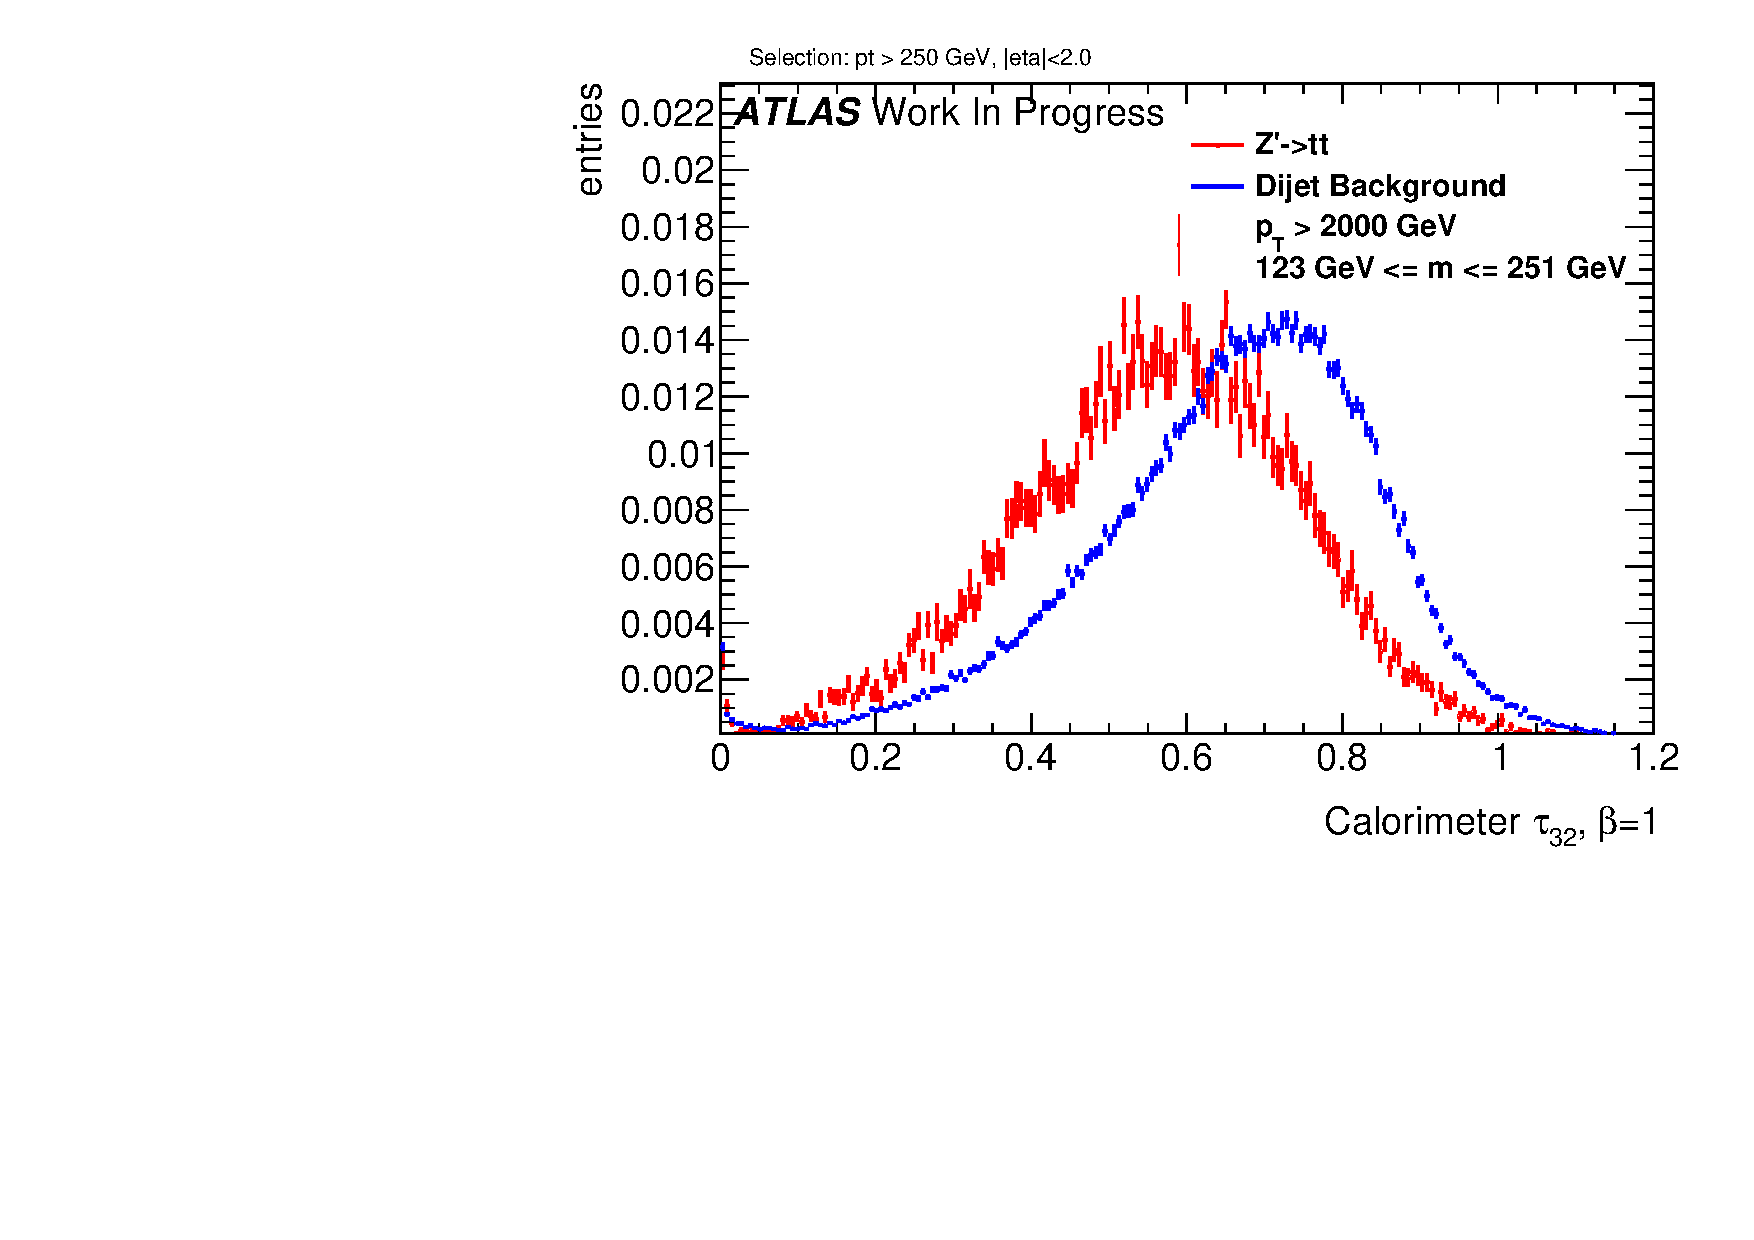
\includegraphics[width=0.6\textwidth]{sascha_input/plots/Top/Beta1/h_recoJet_nSub32_bin6.pdf}
\caption{Exemplary $\tau_{32}$ distributions for Top signal jets and QCD background jets, calculated with clusters. The background tends to higher values.}\label{fig:nSub_example}
\end{figure}

\subsubsection{TAS Procedure for Jet Substructure Observables}
The concept of track assisting with the $p_{\mathrm{T}}$ ratio of the whole jet is without effect for the studied substructure variables. This can be understood from the definitions of the weighted $p_{\mathrm{T}}$ sums. If corrected with only one ratio, all tracks are scaled by the same factor $c$, which then can be put in front of the sum and cancels as soon as the ratios $\tau_{21}$ and $\tau_{32}$, respectively C2 and D2 are formed.
\begin{equation}
\begin{aligned}
 & \tau_N ={} \frac{1}{d_0}\sum_k p_{T,k} \; c \; min(\Delta R_{1,k},\Delta R_{2,k},...,\Delta R_{N,k})^{\beta} \\
 & \; \; \; \;  ={} \frac{c}{d_0}\sum_k p_{T,k}\:min(\Delta R_{1,k},\Delta R_{2,k},...,\Delta R_{N,k})^{\beta}
\end{aligned}
\end{equation}
Track assisting with ghost association to subjets (TAS), see Section \ref{sec:mtas} for $\mtas$, works with different scaling factors depending on the corresponding subjet $c_k$, which also affect ratios:
\begin{equation}
\tau_N = \frac{1}{d_0}\sum_k p_{T,k} \; c_k \; min(\Delta R_{1,k},\Delta R_{2,k},...,\Delta R_{N,k})^{\beta} 
\end{equation}\label{eq:tas_ta}
Therefore for the substructure observables the method used is the TAS, assisting single tracks only as explained in Section \ref{sec:tas}. Tracks and assisted tracks (TAS) as well as calorimeter clusters used as input for these observables are studied. The used selection for tracks is the same as for TAS, only the part of $p_{\text{T}}$ scaling is omitted.
